\clearpage
\section{Apache ZooKeeper}
\label{sec:zookeeper}
We have relied heavily on ZooKeeper in order to store our Voldemort configuration data as well as handling coordination in in our management system. In this section we will explain what ZooKeeper is along with how it works. Finally we will present which techniques we have used along with how we used them. 

\subsection{What is ZooKeeper}
From Apache ZooKeepers own website\cite{zookeeper} they explain ZooKeeper as:

\blockquote{ZooKeeper is a centralized service for maintaining configuration information, naming, providing distributed synchronization, and providing group services. All of these kinds of services are used in some form or another by distributed applications.}

ZooKeeper was designed without specific primitives (i.e. locks and leader election). The reason being that they didn't want to tie down the developer, and instead expose a simple jet powerful API. This allows developers to create their own primitives based on their application specific needs. This means ZooKeeper can be adapted to suit the requirements of different applications. 

\subsection{Clarification}
A \texttt{write} or \texttt{put} in the context of ZooKeeper is considered a ZooKeeper \texttt{setData} operation.

A ZooKeeper event, is an event triggered by a watch set in ZooKeeper, giving push information to a client about a change in ZooKeeper about a znode being watched.

In the context of ZooKeeper, the word file might be used for a znode. File used in the context of a local filesystem is a local file.

\subsection{Znodes}
ZooKeeper behaves almost like a file system with one key difference. Instead of files and directories - we have znodes. All znodes can contain information in the form of bytes. One znodes can have children which again can have more children. Together they form an hierarchical structure, addressable like a unix filesystem path. 

Znodes also include version numbers for data changes, ACL changes and timestamps to allow cache validations as well as coordinate updates. Whenever a znodes data is changed, it's version number increases.

\begin{figure}[h]
    \centering
    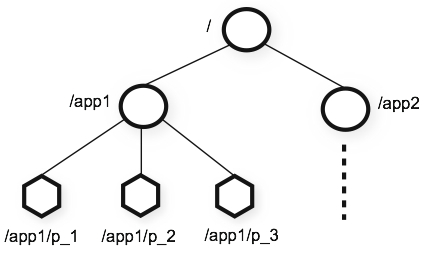
\includegraphics[width=0.4\textwidth]{software/zknamespace.jpg}
    \caption{A sample namespace}
    \label{fig:zk_namespace}
\end{figure}

These znodes can have different flags set which control their behavior. These are \emph{persistent}, \emph{ephemeral} and \emph{sequential}. Persistent is rather self explanatory. When this flag is set during a PUT operation, the data will remain in ZooKeeper even though the client disconnects. Ephemeral is the opposite. Data placed in ZooKeeper with this flag will be deleted when the client ends its session. If sequential is set, each child of the znode will have a monotonic increasing sequence number appended to its path. This number is relative to the parent znode, so children znodes can have equal or different names. Ephemeral and sequential are powerful features which enable us to utilize ZooKeeper for leader election, coordination as well as locks. 

\subsection{ZooKeeper Guarantees}
ZooKeeper provides two basic ordering guarantees:

\begin{itemize}
	\item Asynchronous linearizable writes
 	\item FIFO client order
\end{itemize}

Since we have asynchronous writes a client can have several outstanding operations, but ZooKeeper guarantees that they will be executed in FIFO order. ZooKeeper also provides clients with the option to listen for changes on a znode. ZooKeeper guarantees that a client will receive a changeEvent before see the new state of the system following the change. 

\subsection{Watches}
As mentioned above, a client can request a watch on a znode in ZooKeeper. This watch will give the client a changeEvent the next time this znode is modified. This could be changes in number of children, changes in the data of znode or that the znode has been deleted. These watches can also be put on non existing znodes which gives the client a changeEvent when the znode is registered in ZooKeeper. It is however important to note that a watch will only trigger once, and it is not possible to request infinite watches. So it is up to each individual client to request a new watch after receiving a changeEvent.

Because of ZooKeepers linearizable guarantees a read following one of these watchEvents will always return the new state of the system. In the event of several changes in quick succession it is possible for a client to not be notified of each individual change. It will however always be able to determine the final state of the system after all the changes.

\subsection{Implementation}

As mentioned ZooKeeper can be used for more than just storing configuration data. In this section we will explain some different ways to use ZooKeeper. 

\subsubsection{Group membership}
ZooKeeper can be used to keep track of group membership. To do this we create a znode for the group at a given path. Now members can register their membership by creating a child znode with the \emph{ephemeral} flag set. As long as they have a session with ZooKeeper they will be listed as a member of the group. When a member registers as a child they also put a watch on the parent node. If there is a change in membership, for example when a node is added, then all nodes will receive the changeEvent.

Note that only a message of \emph{change} is delivered. This means that if 3 nodes quickly joins, one watch is delivered for the first change. The client must then query for a new children list. Because of ZooKeepers FIFO ordering guarantees, this request will either include all changes, or the second and third write will trigger a new watch. In effect we will never have the case that when a node is added, and a process watching is not notified. 

\subsubsection{Leader election}
Leader election is something that frequently needs to be addressed in a distributed system. In our own management service we used ZooKeeper to handle this issue. 

To elect a leader we utilize the \emph{sequential} and \emph{ephemeral} flags of a znode. We have a znode called \emph{leaders} in ZooKeeper where potential leaders can register themselves. This znode has the sequential flag set so we get a total order on the potential leaders. We also force each potential leader to use the ephemeral flag when registering. This ensures that when a client disconnects, it is removed from the children list. When it rejoins, it is given a new sequence number. By default the znode with the lowest sequence number will be the one that is the leader.

If a node registers as a potential leader but does not win the election (i.e: There is another contender with a lower sequence number) it puts a watch on the winner and waits for changes. If eventually the leader disconnects then there will once again be elected a new leader based on sequence numbers.

Any client wanting to get a hold of its leader can simply ask ZooKeeper for all the children of the parent znode, and then determine which one is the leader based on sequence numbers. Now the client can put a watch on this leader znode and be notified whenever there is a change in leadership. If said event is received the client simply ask ZooKeeper again for the children and repeat the process. 

This however can cause a thundering horde effect. When the leader disappears, ZooKeeper suddenly have lots of watches to deliver, as well as a horde of incoming requests for children lists of the parent node. To avoid this, every node waiting to be the leader can listen on the \emph{previous} node in the queue. Because of the linearizable guarantees, we know that we will never become the leader until the one in front disappears. This way only one watchEvent has to be delivered, causing only one request for the updated znode list.

\subsubsection{Locks}
Another use case for ZooKeeper is managing limited resources. This is implemented with locks. To create a lock we have a reserved znode for the resource in ZooKeeper. To queue for the lock, clients must create \emph{sequential} and \emph{ephemeral} children on this node. The client with the lowest number holds the lock. We use ephemeral to prevent a client for keeping the lock forever in case of a disconnect, and sequential is for ordering of clients.

It is also possible to separate locks into read and write locks. In ZooKeeper their only difference will be in the naming of the znode, but the client now can regard them as read or write locks. The case explained above is a typical write, or exclusive lock. In the case of a read lock, the client will be allowed access to the resource as long as there is no write locks before it. If there is a write lock ahead of the read, the client will put a watch on the previous exclusive lock and wait until it is deleted. Such read/write locks can typically be created by prepending a ``r'' or an ``x'' on the client znode, to signal a read or exclusive, respectively.



